\chapter{Task 3}

\section{a)}
\begin{center}
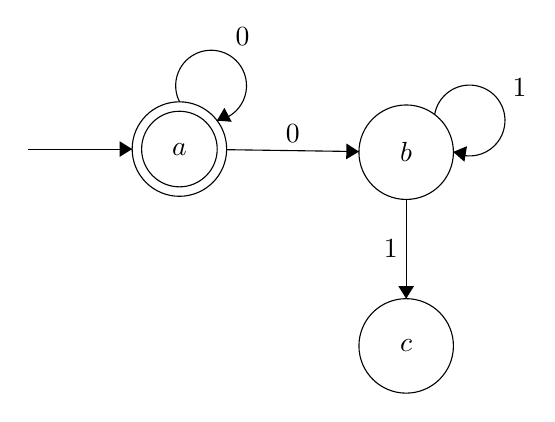
\begin{tikzpicture}[scale=0.2]
\tikzstyle{every node}+=[inner sep=0pt]
\draw [black] (14.9,-15.9) circle (3);
\draw (14.9,-15.9) node {$a$};
\draw [black] (14.9,-15.9) circle (2.4);
\draw [black] (29.3,-16.1) circle (3);
\draw (29.3,-16.1) node {$b$};
\draw [black] (29.3,-28.4) circle (3);
\draw (29.3,-28.4) node {$c$};
\draw [black] (5.3,-15.9) -- (11.9,-15.9);
\fill [black] (11.9,-15.9) -- (11.1,-15.4) -- (11.1,-16.4);
\draw [black] (14.916,-12.912) arc (207.43495:-80.56505:2.25);
\draw (18.91,-9.36) node [above] {$0$};
\fill [black] (17.28,-14.09) -- (18.22,-14.17) -- (17.76,-13.28);
\draw [black] (17.9,-15.94) -- (26.3,-16.06);
\fill [black] (26.3,-16.06) -- (25.51,-15.55) -- (25.49,-16.55);
\draw (22.1,-15.49) node [above] {$0$};
\draw [black] (29.3,-19.1) -- (29.3,-25.4);
\fill [black] (29.3,-25.4) -- (29.8,-24.6) -- (28.8,-24.6);
\draw (28.8,-22.25) node [left] {$1$};
\draw [black] (31.105,-13.719) arc (170.56505:-117.43495:2.25);
\draw (36.03,-11.97) node [right] {$1$};
\fill [black] (32.29,-16.08) -- (33,-16.71) -- (33.16,-15.72);
\end{tikzpicture}
\end{center}
\section{b)}
\begin{center}
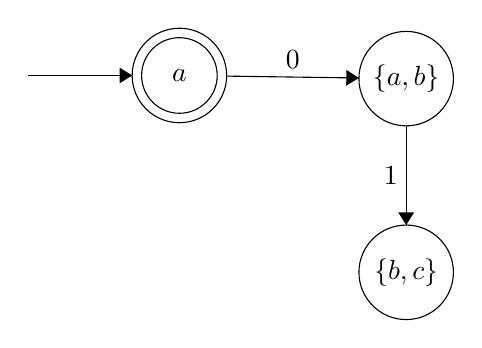
\begin{tikzpicture}[scale=0.2]
\tikzstyle{every node}+=[inner sep=0pt]
\draw [black] (14.9,-15.9) circle (3);
\draw (14.9,-15.9) node {$a$};
\draw [black] (14.9,-15.9) circle (2.4);
\draw [black] (29.3,-16.1) circle (3);
\draw (29.3,-16.1) node {$\{a, b\}$};
\draw [black] (29.3,-28.4) circle (3);
\draw (29.3,-28.4) node {$\{b, c\}$};
\draw [black] (5.3,-15.9) -- (11.9,-15.9);
\fill [black] (11.9,-15.9) -- (11.1,-15.4) -- (11.1,-16.4);
\draw [black] (17.9,-15.94) -- (26.3,-16.06);
\fill [black] (26.3,-16.06) -- (25.51,-15.55) -- (25.49,-16.55);
\draw (22.1,-15.49) node [above] {$0$};
\draw [black] (29.3,-19.1) -- (29.3,-25.4);
\fill [black] (29.3,-25.4) -- (29.8,-24.6) -- (28.8,-24.6);
\draw (28.8,-22.25) node [left] {$1$};
\end{tikzpicture}
\end{center}